\documentclass[11pt,a4paper]{article}

\usepackage[utf8]{inputenc}
\usepackage[T1]{fontenc}
\usepackage{mathpazo}
\usepackage[scaled=0.92]{helvet}
\usepackage[margin=1in]{geometry}
\usepackage{graphicx}
\usepackage{amsmath,amssymb,amsfonts}
\usepackage{booktabs}
\usepackage{tabularx}
\usepackage{setspace}
\usepackage{titlesec}
\usepackage{fancyhdr}
\usepackage{float}
\usepackage{caption}
\usepackage{microtype}

\usepackage{tikz}
\usetikzlibrary{shapes.geometric, arrows.meta, positioning, calc}

\usepackage{listings}
\usepackage{xcolor}
\usepackage[hidelinks]{hyperref}

\setstretch{1.15}
\setlength{\parindent}{0pt}
\setlength{\parskip}{0.8em}
\sloppy

\titleformat{\section}{\normalfont\large\bfseries\sffamily}{\thesection}{1em}{}
\titleformat{\subsection}{\normalfont\normalsize\bfseries\sffamily}{\thesubsection}{1em}{}

\pagestyle{fancy}
\fancyhf{}
\fancyhead[L]{\small\sffamily Fondasi Basis Data: Data Definition Language}
\fancyhead[R]{\small\sffamily\thepage}
\renewcommand{\headrulewidth}{0.4pt}

\captionsetup{font=small,labelfont=bf,labelsep=period}

% Palet warna minimalis untuk kode
\definecolor{codegray}{rgb}{0.5,0.5,0.5}
\definecolor{codeblue}{rgb}{0.1,0.2,0.6}
\definecolor{codebg}{rgb}{0.97,0.97,0.97}

\lstdefinestyle{sqlstyle}{
	backgroundcolor=\color{codebg},
	commentstyle=\color{codegray}\itshape,
	keywordstyle=\color{codeblue}\bfseries,
	numberstyle=\tiny\color{codegray},
	stringstyle=\color{black},
	basicstyle=\ttfamily\small,
	breakatwhitespace=false,
	breaklines=true,
	captionpos=b,
	keepspaces=true,
	numbers=left,
	numbersep=8pt,
	showspaces=false,
	showstringspaces=false,
	showtabs=false,
	tabsize=2,
	frame=single,
	rulecolor=\color{codegray!30},
	language=SQL
}
\lstset{style=sqlstyle}

\renewenvironment{abstract}
{\small
	\begin{center}\textbf{\sffamily Abstrak}\end{center}
	\begin{quote}}
	{\end{quote}}

\title{\vspace{-1.5cm}\textbf{\sffamily\LARGE Fondasi Basis Data: Structured Query Language dan Data Definition Language}}
\author{
	\textbf{Muhammad Riduwan Khafidi} \\
	\small Program Studi Teknik Rekayasa Perangkat Lunak \\
	\small Politeknik Negeri Batam \\
	\small \texttt{4342611034@students.polibatam.ac.id}
}
\date{\small\today}

\begin{document}

\maketitle
\thispagestyle{empty}

\begin{abstract}
	Structured Query Language (SQL) merupakan bahasa standar yang digunakan untuk berkomunikasi dengan sistem manajemen basis data relasional (RDBMS). Sejak distandarisasi oleh ANSI, SQL telah menjadi tulang punggung dalam pengelolaan data modern, terbagi menjadi tiga pilar utama: Data Definition Language (DDL), Data Manipulation Language (DML), dan Data Control Language (DCL). Makalah ini membedah secara mendalam konsep DDL, yang berperan sebagai fondasi dalam mendefinisikan struktur basis data. Pembahasan mencakup tipologi tipe data, pembuatan tabel (CREATE), penerapan batasan integritas (Integrity Constraints) seperti Primary Key dan Foreign Key, modifikasi struktur (ALTER), hingga optimalisasi pencarian data menggunakan Index. Selain itu, makalah ini juga menyentuh dasar-dasar manipulasi data (CRUD) untuk memberikan gambaran utuh mengenai siklus hidup data di dalam basis data.
\end{abstract}

\section{Pendahuluan: Bahasa Universal Basis Data}

Bayangkan sebuah perusahaan raksasa seperti Oracle, Microsoft, atau Meta. Mereka memiliki sistem basis data yang berbeda-beda, namun para *programmer* mereka dapat berbicara dalam satu bahasa yang sama: \textbf{SQL (Structured Query Language)}. Menurut American National Standards Institute (ANSI), SQL adalah bahasa standar untuk sistem manajemen basis data relasional.

Sejarah SQL tidak lepas dari peran Dr. Edgar F. Codd dari IBM pada tahun 1970 yang mencetuskan model relasional. Ide tersebut diwujudkan dalam bentuk bahasa pada tahun 1974, dan pada tahun 1986 distandarisasi oleh ANSI. Meskipun setiap RDBMS (seperti MySQL, PostgreSQL, Oracle, SQL Server) memiliki ekstensi tambahan (dialek) masing-masing, perintah standar seperti \texttt{SELECT}, \texttt{INSERT}, \texttt{UPDATE}, \texttt{DELETE}, \texttt{CREATE}, dan \texttt{DROP} berlaku universal.

\section{Tiga Pilar SQL}

Dalam praktiknya, SQL tidak hanya digunakan untuk mengambil data, tetapi juga untuk membangun struktur dan mengatur keamanan. Secara garis besar, SQL terbagi menjadi tiga bagian yang saling melengkapi, seperti yang diilustrasikan pada Gambar \ref{fig:sql_parts}.

\begin{figure}[H]
	\centering
	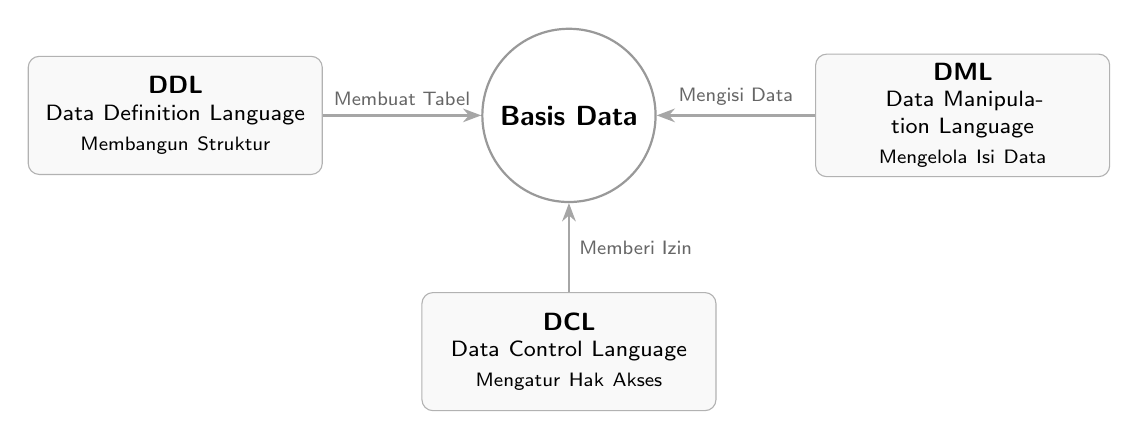
\begin{tikzpicture}[
			box/.style={draw=gray!60, rectangle, rounded corners=4pt, text width=3.5cm, align=center, minimum height=1.5cm, font=\sffamily\small, fill=gray!5},
			arrow/.style={->, >=Stealth, thick, color=gray!70}
		]
		% DDL
		\node[box] (ddl) at (0,0) {\textbf{DDL}\\ \footnotesize Data Definition Language\\ \scriptsize Membangun Struktur};

		% DML
		\node[box] (dml) at (10,0) {\textbf{DML}\\ \footnotesize Data Manipulation Language\\ \scriptsize Mengelola Isi Data};

		% DCL
		\node[box] (dcl) at (5,-3) {\textbf{DCL}\\ \footnotesize Data Control Language\\ \scriptsize Mengatur Hak Akses};

		% Central Concept
		\node[draw=gray!80, circle, fill=white, thick, minimum size=2.2cm, font=\bfseries\sffamily] (db) at (5,0) {Basis Data};

		\draw[arrow] (ddl) -- (db) node[midway, above, font=\scriptsize\sffamily, color=gray!80!black] {Membuat Tabel};
		\draw[arrow] (dml) -- (db) node[midway, above, font=\scriptsize\sffamily, color=gray!80!black] {Mengisi Data};
		\draw[arrow] (dcl) -- (db) node[midway, right, font=\scriptsize\sffamily, color=gray!80!black] {Memberi Izin};
	\end{tikzpicture}
	\caption{Ilustrasi Tiga Pilar Utama dalam SQL.}
	\label{fig:sql_parts}
\end{figure}

Pilar pertama adalah \textbf{DDL}, yang berfungsi seperti seorang arsitek. Ia mendefinisikan skema, domain, batasan integritas, hingga struktur penyimpanan fisik. Pilar kedua adalah \textbf{DML}, yang berfungsi seperti pekerja. Ia melakukan *query* dan pembaruan data (CRUD). Pilar ketiga adalah \textbf{DCL}, yang berfungsi seperti satpam. Ia mengatur siapa saja yang boleh mengakses dan memodifikasi data (misalnya melalui perintah \texttt{GRANT} dan \texttt{REVOKE}). Makalah ini akan berfokus pada pilar pertama, yaitu DDL.

\section{Memahami Tipe Data (Domain Types)}

Sebelum membangun tabel, seorang perancang harus memahami tipe data apa yang akan digunakan. Salah satu pertanyaan klasik adalah perbedaan antara \texttt{CHAR(n)} dan \texttt{VARCHAR(n)}.

\texttt{CHAR(n)} adalah *fixed-length string* (panjang tetap). Jika kita mendeklarasikan \texttt{CHAR(10)} dan menyimpan kata ``du'', sistem tetap akan mengalokasikan 10 *byte* memori (kekurangannya diisi spasi). Sementara itu, \texttt{VARCHAR(n)} adalah *variable-length string*. Jika kita menyimpan ``du'' di \texttt{VARCHAR(10)}, sistem hanya akan mengalokasikan memori sesuai panjang karakternya (plus sedikit *overhead*). Perbedaan ini berdampak besar pada efisiensi ruang penyimpanan seperti yang terlihat pada tabel di bawah ini.

\begin{table}[H]
	\centering
	\small
	\caption{Perbandingan Alokasi Memori \texttt{CHAR(10)} vs \texttt{VARCHAR(10)}}
	\label{tab:char_varchar}
	\begin{tabularx}{0.7\textwidth}{@{} X c c @{}}
		\toprule
		\textbf{Data yang Disimpan} & \textbf{Memori \texttt{CHAR(10)}} & \textbf{Memori \texttt{VARCHAR(10)}} \\
		\midrule
		``du''                      & 10 bytes                          & 2 bytes                              \\
		``dunia''                   & 10 bytes                          & 5 bytes                              \\
		``duniaku''                 & 10 bytes                          & 7 bytes                              \\
		\bottomrule
	\end{tabularx}
\end{table}

Selain teks, SQL menyediakan tipe angka presisi (\texttt{INTEGER}, \texttt{NUMERIC(p,d)}), angka desimal mengambang (\texttt{REAL}, \texttt{FLOAT}), waktu (\texttt{DATE}, \texttt{TIME}, \texttt{TIMESTAMP}), serta tipe \texttt{NULL} yang merepresentasikan ketiadaan nilai. Jika sebuah atribut dideklarasikan \texttt{NOT NULL}, maka atribut tersebut wajib memiliki nilai.

\section{Membangun Struktur: CREATE TABLE}

Pilar utama DDL adalah perintah \texttt{CREATE TABLE}. Bayangkan kita ingin membuat sistem perbankan sederhana. Kita bisa membuat tabel \texttt{branch} (cabang bank) dengan sintaks berikut.

\begin{lstlisting}
CREATE TABLE branch (
    branch_name VARCHAR(15) NOT NULL,
    branch_city VARCHAR(30),
    assets INTEGER,
    PRIMARY KEY (branch_name),
    CHECK (assets >= 0)
);
\end{lstlisting}

Dalam perintah di atas, kita tidak hanya mendefinisikan kolom dan tipe datanya, tetapi juga menerapkan \textbf{Integrity Constraints} (Batasan Integritas):

\textbf{NOT NULL} memastikan kolom \texttt{branch\_name} tidak boleh kosong. \textbf{PRIMARY KEY} menetapkan bahwa \texttt{branch\_name} harus unik dan menjadi identitas utama baris tersebut. \textbf{CHECK} memastikan bahwa nilai \texttt{assets} (aset) tidak boleh bernilai negatif. Jika ada upaya memasukkan aset minus, sistem akan menolak secara otomatis.

\subsection{Relasi Antar Tabel: Foreign Key dan CASCADE}
Dalam basis data relasional, tabel tidak berdiri sendiri. Kita sering menghubungkan tabel \texttt{borrower} (peminjam) dengan tabel \texttt{customer} dan \texttt{loan}.

\begin{lstlisting}
CREATE TABLE borrower (
    customer_name VARCHAR(30),
    loan_number NUMBER(8),
    PRIMARY KEY (customer_name, loan_number),
    FOREIGN KEY (customer_name) REFERENCES customer(customer_name),
    FOREIGN KEY (loan_number) REFERENCES loan(loan_number) ON DELETE CASCADE
);
\end{lstlisting}

Perhatikan penggunaan \textbf{FOREIGN KEY} (Kunci Tamu). Ia memastikan bahwa data peminjam yang dimasukkan benar-benar terdaftar di tabel \texttt{customer}.

Konsep krusial di sini adalah \textbf{ON DELETE CASCADE}. Tanpa pengaturan ini, jika kita menghapus data \texttt{customer} dari tabel utama, sistem akan kebingungan karena datanya masih dipakai di tabel \texttt{borrower}. Dengan \texttt{CASCADE}, jika data \texttt{customer} dihapus, maka semua data pinjaman milik *customer* tersebut di tabel \texttt{borrower} akan ikut terhapus secara otomatis untuk menjaga integritas data.

\section{Modifikasi Struktur: ALTER TABLE}

Seiring berjalannya waktu, kebutuhan bisnis berubah. DDL menyediakan perintah \texttt{ALTER TABLE} untuk memodifikasi tabel yang sudah ada tanpa harus menghapus dan membuatnya ulang.

Jika kita ingin menambahkan kolom baru (misalnya tanggal lahir peminjam), kita gunakan \texttt{ALTER TABLE borrower ADD b\_date DATE;}. Jika ingin mengganti nama kolom, gunakan \texttt{ALTER TABLE borrower CHANGE b\_date birth\_date DATE;}. Jika kolom tersebut sudah tidak relevan, hapus dengan \texttt{ALTER TABLE borrower DROP birth\_date;}. Kita juga dapat menambahkan \texttt{DEFAULT} value, misalnya \texttt{Gender CHAR(1) DEFAULT '?'} jika gender tidak diisi.

\section{Optimalisasi Pencarian: Index}

Bayangkan sebuah tabel berisi jutaan data nasabah. Jika kita sering mencari data berdasarkan nama cabang (\texttt{branch\_name}), proses pencarian akan memakan waktu lama. Di sinilah \textbf{INDEX} berperan. Index bekerja seperti indeks di bagian belakang sebuah buku. Sistem tidak perlu membaca seluruh halaman, cukup melihat indeks untuk langsung melompat ke halaman yang dituju.

\begin{figure}[H]
	\centering
	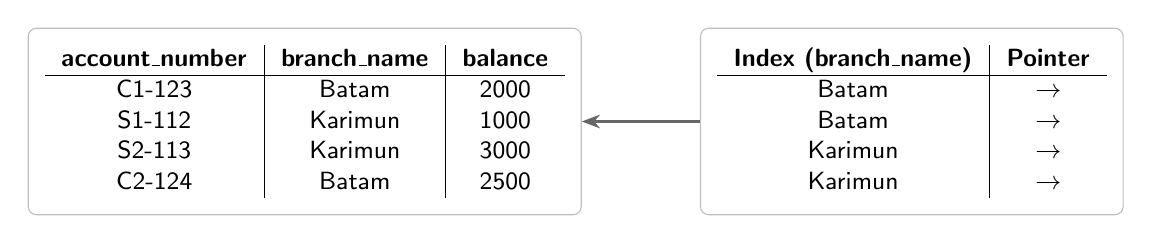
\begin{tikzpicture}[
			box/.style={draw=gray!50, rectangle, rounded corners=3pt, fill=white, inner sep=6pt, font=\small\sffamily},
			header/.style={font=\small\sffamily\bfseries},
			arrow/.style={->, >=Stealth, thick, color=gray!80!black}
		]
		% Tabel Fisik
		\node[box] (tbl) {
			\begin{tabular}{c|c|c}
				\textbf{account\_number} & \textbf{branch\_name} & \textbf{balance} \\
				\hline
				C1-123                   & Batam                 & 2000             \\
				S1-112                   & Karimun               & 1000             \\
				S2-113                   & Karimun               & 3000             \\
				C2-124                   & Batam                 & 2500             \\
			\end{tabular}
		};

		% Indeks
		\node[box, right=1.5cm of tbl] (idx) {
			\begin{tabular}{c|c}
				\textbf{Index (branch\_name)} & \textbf{Pointer} \\
				\hline
				Batam                         & \(\rightarrow\)  \\
				Batam                         & \(\rightarrow\)  \\
				Karimun                       & \(\rightarrow\)  \\
				Karimun                       & \(\rightarrow\)  \\
			\end{tabular}
		};

		\draw[arrow] (idx.west) -- (tbl.east);
	\end{tikzpicture}
	\caption{Ilustrasi Index yang Menunjuk Langsung ke Baris Data.}
	\label{fig:index}
\end{figure}

Seperti yang terlihat pada Gambar \ref{fig:index}, dengan membuat \texttt{CREATE INDEX branch\_idx ON Account (branch\_name)}, sistem akan membuat daftar terurut. Pencarian kata ``Karimun'' akan langsung menunjuk ke barisnya tanpa memindai seluruh tabel.

Namun, Index memiliki harga. \textbf{Jangan gunakan Index} pada tabel yang sangat kecil, pada kolom yang isinya didominasi oleh nilai \texttt{NULL}, atau pada tabel yang sangat sering mengalami operasi \texttt{UPDATE} dan \texttt{INSERT} secara masif. Setiap kali data ditambahkan atau diubah, sistem harus memperbarui Index-nya juga, yang justru memperlambat proses penulisan.

\section{Data Manipulation (CRUD) sebagai Pelengkap}

Setelah struktur (DDL) selesai dibangun, data di dalamnya diisi dan dikelola menggunakan DML. Operasi dasar CRUD (*Create, Read, Update, Delete*) dijalankan melalui perintah berikut.

Untuk menambah data baru, digunakan \texttt{INSERT INTO account VALUES ('A-9732', 'Perryridge', 1200);}. Jika urutan kolom tidak diingat, kita bisa spesifikasikan: \texttt{INSERT INTO account (branch\_name, balance, account\_number) VALUES ('Perryridge', 1200, 'A-9732');}.

Untuk menghapus data spesifik, perintah \texttt{DELETE FROM account WHERE branch\_name = 'Perryridge';} akan menghapus baris dengan kondisi tertentu. Namun, perintah \texttt{DELETE FROM account;} tanpa klausa \texttt{WHERE} akan mengosongkan seluruh tabel.

Adapun untuk mengubah data, digunakan \texttt{UPDATE}. Misalnya, jika bank ingin memberikan bunga 5\% untuk nasabah dengan saldo di atas 1000, perintahnya adalah \texttt{UPDATE account SET balance = balance * 1.05 WHERE balance > 1000;}.

Menariknya, SQL juga mendukung logika percabangan menggunakan \texttt{CASE}. Jika bank ingin memberikan bunga 6\% untuk saldo di atas 1000, dan 5\% untuk saldo di bawahnya, hal ini bisa dilakukan dalam satu perintah *update*:

\begin{lstlisting}
UPDATE account
SET balance = CASE
    WHEN balance <= 1000 THEN balance * 1.05
    ELSE balance * 1.06
END;
\end{lstlisting}

\section{Kesimpulan}

Data Definition Language (DDL) adalah fondasi yang menentukan seberapa kokoh sebuah sistem basis data. Melalui pemilihan tipe data yang tepat (seperti \texttt{CHAR} vs \texttt{VARCHAR}), penerapan *constraints* yang ketat (seperti \texttt{PRIMARY KEY}, \texttt{FOREIGN KEY}, dan \texttt{CASCADE}), serta strategi *Indexing* yang bijak, seorang perancang dapat memastikan bahwa data tidak hanya tersimpan dengan aman, tetapi juga dapat diakses dengan sangat cepat. Penguasaan DDL, yang dilengkapi dengan pemahaman dasar DML, adalah bekal mutlak bagi setiap *software engineer* dalam membangun aplikasi berskala besar.

\newpage
\section*{Referensi}
\addcontentsline{toc}{section}{Referensi}

\begin{thebibliography}{99}
	\bibitem{lubis}
	Lubis, A. I. (2026). \textit{Data Definition Language} [Slide Presentasi Mata Kuliah Pengantar Basis Data]. Politeknik Negeri Batam.

	\bibitem{silberschatz}
	Silberschatz, A., Korth, H. F., \& Sudarshan, S. (2019). \textit{Database System Concepts} (7th ed.). McGraw-Hill Education.
\end{thebibliography}

\end{document}
